The following records, documented in Chapter \ref{ch-network} are used by Helios:
\begin{itemize}
\item[] BUS
\item[] BUSDC
\item[] LINE
\item[] SWITCH
\item[] TRANSFO
\item[] TRFO
\item[] NRTP.
\end{itemize}

The additional (mandatory or optional) records only used in power flow computations are documented in this chapter.

\section{Load and shunt data}\label{sec-pf-bus}

Load and shunt data are attached to buses. They are specified in an extended version of the BUS record, as follows:

\hspace*{5ex}{\tt BUS NAME VNOM PLOAD QLOAD BSHUNT QSHUNT ;}

where:
\begin{itemize}
\item {\tt NAME} is the name of the bus. This is a string of at most 8 characters
\item {\tt VNOM} is the nominal voltage, in kV
\item {\tt PLOAD} is the total active power load at the bus, in MW. A positive value corresponds to power drawn from the network
\item {\tt QLOAD} is the total reactive power load at the bus, in Mvar. A positive value corresponds to power drawn from the network
\item {\tt BSHUNT} is the nominal reactive power of the shunt modelled as constant susceptance, in Mvar. This is the reactive power produced by the shunt under the nominal voltage of the bus, specified in its BUS record. BSHUNT is positive (resp. negative) for a shunt capacitor (resp. inductor)
\item {\tt QSHUNT} is the reactive power produced by the shunt modelled as constant power, in Mvar. QSHUNT is positive (resp. negative) for a shunt capacitor (resp. inductor).
\end{itemize}

The total reactive power $Q$ produced by the two shunt components is given, in Mvar, by:
\[ Q = BSHUNT \; (\frac{V}{V_{nom}})^2 + QSHUNT \]
where $V$ is the bus voltage and $V_{nom}$ the corresponding nominal voltage.

If no shunt is connected to the bus, BSHUNT and QSHUNT are set to zero.

If no load is connected to the bus, PLOAD and QLOAD are set to zero.

Let us recall that the PLOAD, QLOAD, BSHUNT and QSHUNT fields are ignored by RAMSES.


%----------------------------------------------------------------------------------
\section{Generator data}

Generators are specified by GENER records, as follows:

\hspace*{5ex}{\tt GENER NAME BUS P Q VIMP SNOM QMIN QMAX BR ;}

where:
\begin{itemize}
\item {\tt NAME} is the name of the generator. This is a string of a most 20 characters
\item {\tt BUS} is the name of the bus which the generator is connected to. This is a string of at most 8 characters
\item {\tt P} is the  active power produced by the generator, in MW
\item {\tt Q} is the reactive power produced by the generator, in Mvar. This value is ignored if the {\tt VIMP} field is nonzero
\item {\tt VIMP} is the voltage imposed by the generator, in pu. If {\tt VIMP} is zero, the bus is
treated as a PQ bus with the reactive power production set to {\tt Q}; if {\tt VIMP} is nonzero, the bus is treated as a PV bus and the {\tt Q} field is ignored
\item {\tt SNOM} is the nominal apparent power of the generator, in MVA
\item {\tt QMIN} is the lower reactive power limit, in Mvar. It is used only if {\tt VIMP} is nonzero
\item {\tt QMAX} is the upper reactive power limit, in Mvar. It is used only if {\tt VIMP} is nonzero
\item {\tt BR} is the on/off status of the generator breaker. A zero value indicates that the
breaker is open; any other value means that the breaker is closed.
\end{itemize}

For all generators with a nonzero value of {\tt VIMP}, the connection bus is initially assumed of the PV type.

If this entails exceeding the generator upper reactive power limit {\tt QMAX}, the bus switches to PQ type, the {\tt QMAX} limit is enforced, and Newton iterations continue. If subsequently the bus voltage gets larger than {\tt VIMP}, the bus switches back to PV type with the voltage imposed at the {\tt VIMP} value.

Similarly, if the generator lower reactive power limit {\tt QMIN} is exceeded, the bus switches to PQ type, the {\tt QMIN} limit is enforced, and Newton iterations continue. If subsequently the bus voltage gets smaller than {\tt VIMP}, the bus switches back to PV type with the voltage imposed at the {\tt VIMP} value.

Only one generator is allowed per bus.

All generators are memorized, even those which are disconnected. A disconnected generator is not involved  (it appears in the output results with a zero power output) but it can be put into service in the
dynamic simulation.

{\bf \large Remark 1}. For simplicity, a generator producing constant active and reactive powers can be modelled as a negative load using the BUS and no GENER record.

{\bf \large Remark 2}. There exists a variant of the GENER record with the following syntax:

\hspace*{5ex}{\tt GENER NAME BUS P Q V SNOM QMIN QMAX PMIN PMAX BR ;}

where {\tt PMIN} (resp. {\tt PMAX}) is the minimum (resp. maximum) active power that the generator can produce, in MW. If this record is present in the data, the {\tt PMIN} and {\tt PMAX} fields are ignored by STEPSS.


%----------------------------------------------------------------------------------
\section{Slack-bus specification}\label{sec-pf-slack}

The presence of a slack-bus is mandatory in power flow computations: indeed, not all buses can be of the PV or PQ type, since this would entail specifying the active power losses in the network, which are not known before performing the power flow calculation.

A generator of the PV type must be connected to the slack-bus. Its voltage magnitude, specified in its GENER record, is imposed at the bus, while the voltage phase angle is set to zero.

A SLACK record may appear once per AC island, where an island is a set of AC buses joined by in-service branches; two SLACK records in one island are an error. SLACK records in separate AC islands are each solved, each slack generator balancing its own island, and the power balance reports the sum over all slack generators.

An island without a SLACK takes as its reference the first in-service AC/DC converter on it (Section~\ref{sec-pf-acdc}), in record order, with {\tt VAC} given; that converter must have {\tt VDC} {\tt *}, and the log names it. Islands with neither a SLACK nor such a converter are ignored with a warning. Only islands with a reference, and the DC grids their converters energise, are solved.

The SLACK record allows specifying which bus is the slack-bus. The syntax is as follows:

\hspace*{5ex}{\tt SLACK NAME ;}

where {\tt NAME} is the name of the bus. This is a string of at most 8 characters.

At least one SLACK record is required.

%----------------------------------------------------------------------------------
\section{Static Var Compensators}

\subsection{Modelling}

The Static Var Compensator (SVC) is modelled as shown in Fig.~\ref{fig-pf-SVC}. $j$ is the {\sl \large monitored } bus, whose voltage is regulated, while $i$ is the {\sl \large controlled} bus, where the shunt susceptance $B$ is varied. $i$ and $j$ can be any two buses but usually $j$ is the transmission bus on the high-voltage side of the SVC step-up transformer, while the SVC is connected to bus $i$.

\begin{figure}[h!]
\centering
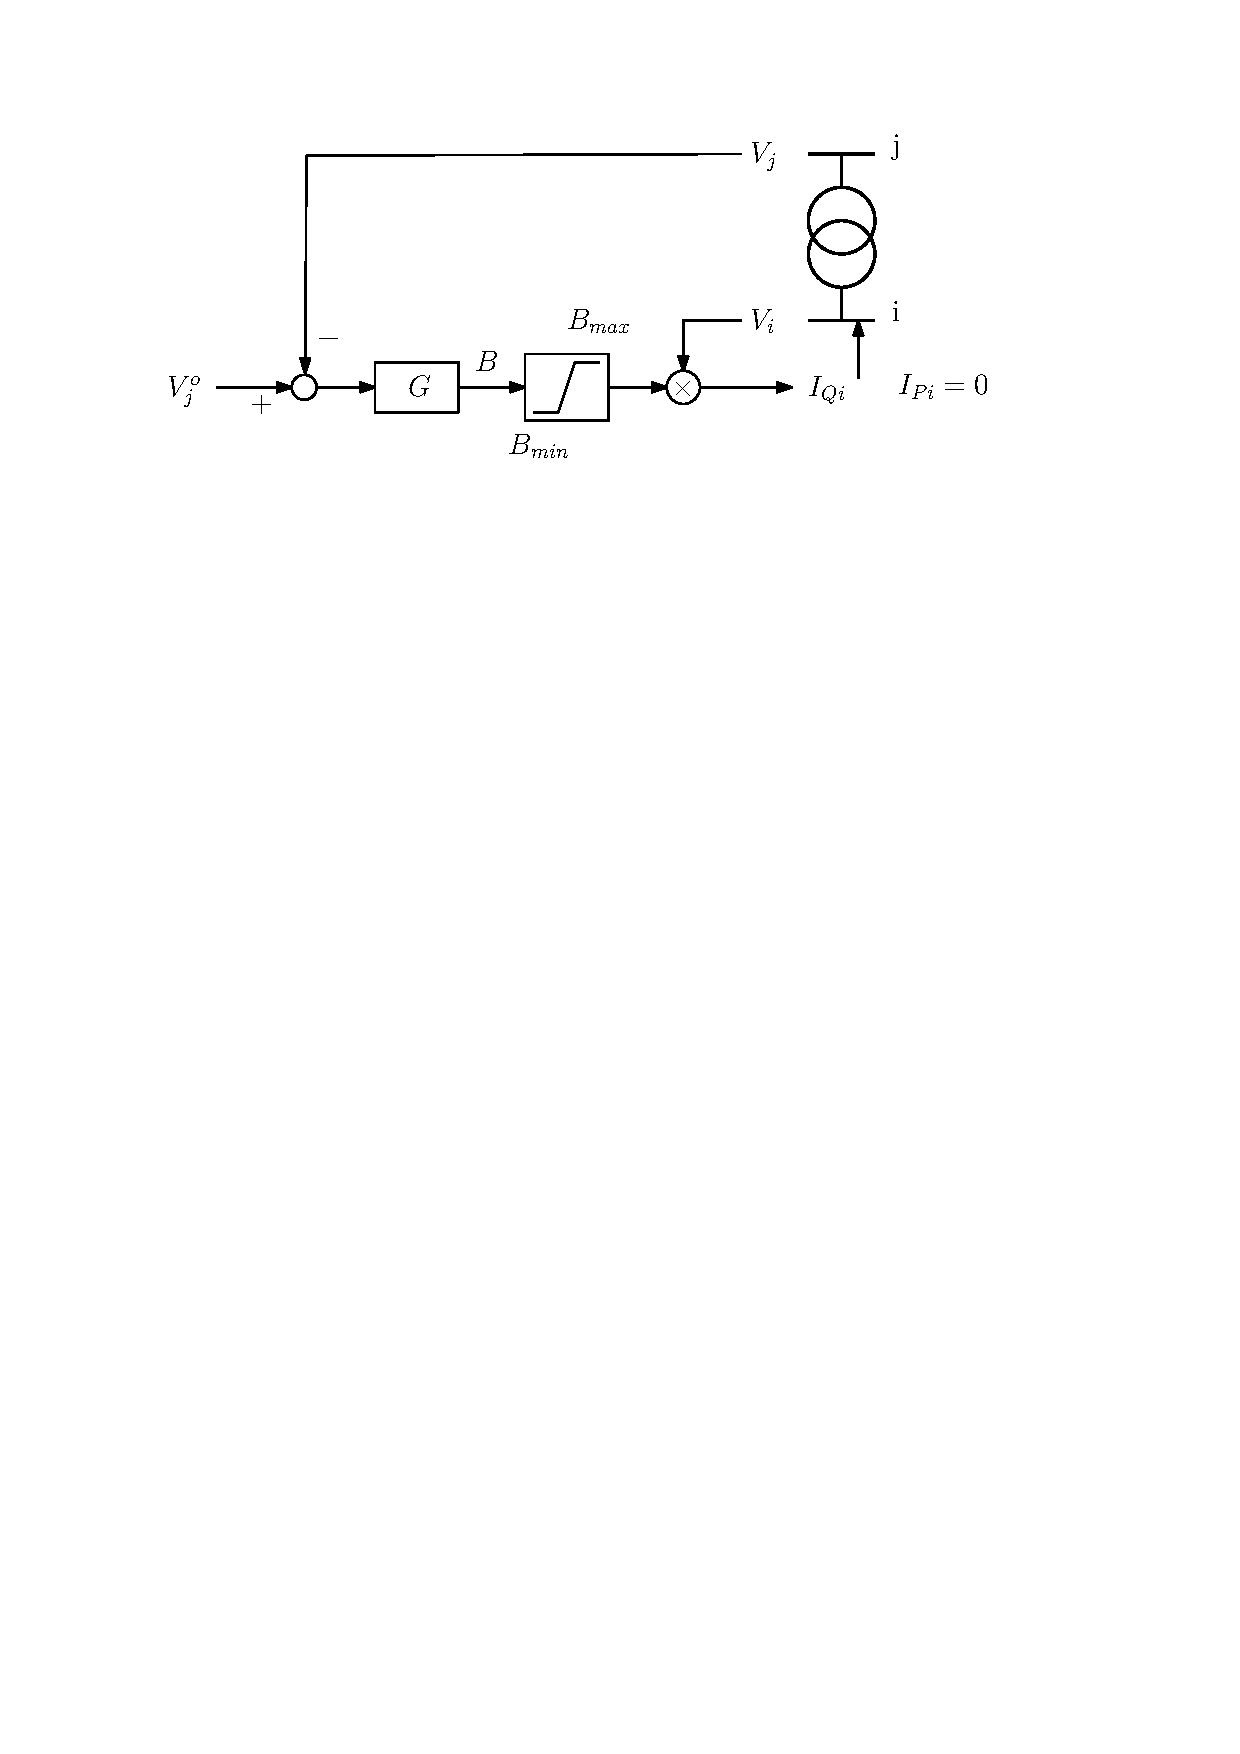
\includegraphics[scale=0.8]{SVC.pdf}
\caption{Block-diagram of the static var compensator}\label{fig-pf-SVC}
\end{figure}

The SVC being assumed lossless, the active current injected at bus $i$ is zero ($I_{Pi} = 0$), while the reactive current takes on one of the following forms:
\begin{eqnarray}
I_{Qi} & = & B V_i = G (V_j^o - V_j) V_i \;\;\;\; \mbox{under voltage control} \label{eq-svc-vcontrol} \\
I_{Qi} & = & B_{max} V_i \;\;\;\; \mbox{under upper susceptance limit} \label{eq-svc-Bmax}\\
I_{Qi} & = & B_{min} V_i \;\;\;\; \mbox{under lower susceptance limit.} \label{eq-svc-Bmin}
\end{eqnarray}

Although reference is made to an SVC, the model can be used in general for a component controlling voltage with a droop.

\subsection{Data format}

The record, with keyword SVC, includes the following fields:

\hspace*{5ex}{\tt SVC NAME CON\_BUS MON\_BUS V0 Q0 SNOM BMAX BMIN G BR ;}

where:
\begin{itemize}
\item {\tt NAME} is the name of the compensator. This is a string of a most 20 characters
\item {\tt CON\_BUS} is the name of the controlled bus. This is a string of a most 8 characters
\item {\tt MON\_BUS} is the name of the monitored bus. This is a string of a most 8 characters
\item {\tt V0} is the voltage setpoint $V_j^o$, in pu (see Fig.~\ref{fig-pf-SVC}) 
\item {\tt Q0} is the reactive power setpoint, in Mvar. If {\tt V0} is set to zero, the SVC is treated under constant power, with $P = 0$ and $Q = Q0$, and no limit is
tested. If {\tt V0} is nonzero, the {\tt Q0} field is ignored
\item {\tt SNOM} is the nominal reactive power of the SVC, in Mvar
\item {\tt BMAX} is the maximal nominal reactive power, in Mvar. This is the reactive 
power produced by the compensator under $V_i = 1$~pu, when $B$ is at
the maximal value $B_{max}$.
\item {\tt BMIN} is the minimal nominal reactive power, in Mvar. This is the reactive
produced by the compensator under $V_i = 1$~pu, when $B$ is at
the minimal value $B_{min}$.
\item {\tt G} is the gain $G$, in pu on the ($V_B$, {\tt SNOM}) base, where $V_B$ is the nominal voltage at the controlled bus, as given by its BUS record
\item {\tt BR} is the on/off status of the SVC breaker. A zero value indicates that
the breaker is open, any other value means that it is closed.
\end{itemize}

It is common for {\tt BMAX} to be positive and {\tt BMIN} negative but other combinations are allowed.

For all SVCs with a nonzero value of {\tt V0}, Eq.~(\ref{eq-svc-vcontrol}) is solved initially.

If this entails exceeding the susceptance upper reactive power limit {\tt BMAX}, Eq.~(\ref{eq-svc-Bmax}) is substituted, the {\tt BMAX} limit is enforced, and Newton iterations continue. If subsequently $G(V_j^o-V_j)< B_{max}$, the program reverts to Eq.~\ref{eq-svc-vcontrol} and keeps on iterating.

Similarly, if the SVC lower suscepance limit {\tt BMIN} is exceeded, Eq.~(\ref{eq-svc-Bmin}) is substituted, the {\tt BMIN} limit is enforced, and Newton iterations continue. If subsequently $G(V_j^o-V_j) > B_{min}$, the program reverts to Eq.~(\ref{eq-svc-vcontrol}) and keeps on iterating.

Only one SVC is allowed per bus. 

It is not allowed to connect both a generator and an SVC to the same bus.

All SVCs are memorized, even those which are disconnected. A disconnected SVC is not involved (it appears in the output results with a zero power output) but it can be put into service in the
dynamic simulation.


%----------------------------------------------------------------------------------
\section{AC/DC converters}\label{sec-pf-acdc}

Helios solves a combined AC-DC power flow: the AC network, the DC buses (Section~\ref{sec-netw-busdc}) and DC lines (Section~\ref{sec-netw-dcline}) of one or more DC grids, and the static converters joining them are solved together in the same Newton iteration. The ACDC record describes a voltage-source converter between an AC bus and a DC bus, with optional DC voltage droop, quadratic converter losses and a converter station. It is read from Helios 1.6.0 onward.

\subsection{Modelling}

The AC bus of the record is the point of common coupling (PCC), where the AC set-points apply. Without a station the converter sits directly at the PCC. With a station, a transformer ($R_{TF} + jX_{TF}$) runs from the PCC to a filter node carrying the filter susceptance $B_F$, and a phase reactor ($R_C + jX_C$) runs from the filter node to the converter node, whose voltage is $V_c$ and whose power into the converter is $P_c + jQ_c$. The losses of the conversion itself sit between the converter node and the DC bus.

\subsection{Data format}

The record always carries all 26 fields. A {\tt *} marks a field that is free or absent; what {\tt *} means is given for each field.

\hspace*{5ex}{\tt ACDC NAME ACBUS DCBUS PAC QAC VAC PDC VDC EFF QMIN QMAX KDROOP DVDB}\\
\hspace*{10ex}{\tt PMIN PMAX LOSSA LOSSB LOSSCR LOSSCI KVC RTF XTF BF RC XC BR ;}

where:
\begin{itemize}
\item {\tt NAME} is the converter name, unique (required)
\item {\tt ACBUS} is the AC bus, the PCC (required)
\item {\tt DCBUS} is the DC bus, declared by a BUSDC record (required)
\item {\tt PAC} is the active power drawn from the AC grid at the PCC, in MW, positive when rectifying ({\tt *}: free)
\item {\tt QAC} is the reactive power injected into the AC grid at the PCC, in Mvar ({\tt *}: 0 when fixed)
\item {\tt VAC} is the AC voltage set-point at the PCC, in pu ({\tt *}: no AC voltage control)
\item {\tt PDC} is the active power delivered into the DC bus, in MW, positive when rectifying; for a droop converter, the power set-point $P_{SET}$ ({\tt *}: free)
\item {\tt VDC} is the DC voltage set-point, in pu; for a droop converter, the voltage set-point $V_{SET}$ ({\tt *}: no DC voltage control)
\item {\tt EFF} is the efficiency, in pu, with $0 < \mbox{EFF} \le 1$ ({\tt *}: use the LOSS fields)
\item {\tt QMIN}, {\tt QMAX} are the lower and upper reactive limits at the PCC, in Mvar, used with {\tt VAC} ({\tt *}: no limit on that side)
\item {\tt KDROOP} is the droop gain, in MW of {\tt PDC} change per pu of DC voltage, $> 0$ ({\tt *}: no droop)
\item {\tt DVDB} is the symmetric deadband around {\tt VDC}, in pu, $\ge 0$ ({\tt *}: 0)
\item {\tt PMIN}, {\tt PMAX} are the lower and upper {\tt PDC} limits of a droop converter, in MW ({\tt *}: no limit on that side)
\item {\tt LOSSA} is the constant loss, in MW ({\tt *}: use {\tt EFF})
\item {\tt LOSSB} is the linear loss coefficient, in kV, which multiplies the converter current ({\tt *}: use {\tt EFF})
\item {\tt LOSSCR}, {\tt LOSSCI} are the quadratic loss coefficients, in ohm, which multiply the current squared, when the converter is physically rectifying and inverting respectively ({\tt *}: use {\tt EFF})
\item {\tt KVC} is the converter-side line voltage base for the loss current, in kV, $> 0$ ({\tt *}: VNOM of {\tt ACBUS})
\item {\tt RTF}, {\tt XTF} are the station transformer resistance and reactance, PCC to filter node, in pu ({\tt *}: absent)
\item {\tt BF} is the filter susceptance at the filter node, in pu, capacitive positive ({\tt *}: absent)
\item {\tt RC}, {\tt XC} are the phase reactor resistance and reactance, filter node to converter node, in pu ({\tt *}: absent)
\item {\tt BR} is the status: 1 in service, 0 out of service (required).
\end{itemize}

Powers are divided by the base power $S_B$ ({\tt \$SBASE}). The station impedances and {\tt BF} are in pu on $S_B$ and the VNOM of {\tt ACBUS}. With every station field {\tt *}, the converter node is the PCC.

\subsection{Control modes}

{\bf AC side}, from {\tt VAC}. With {\tt VAC} {\tt *}, {\tt QAC} is fixed (PQ). With {\tt VAC} given, the PCC is a PV bus and {\tt QAC} floats between {\tt QMIN} and {\tt QMAX}. {\tt QMIN} greater than {\tt QMAX} is an error.

{\bf DC side}, from {\tt VDC} and {\tt KDROOP}:
\begin{itemize}
\item both {\tt *}: {\sl fixed power}. One of {\tt PAC} and {\tt PDC} is given and the other follows;
\item {\tt VDC} given, {\tt KDROOP} {\tt *}: {\sl constant DC voltage}. The DC bus is held at {\tt VDC} and the power floats; any {\tt PAC} or {\tt PDC} given is only a starting guess;
\item {\tt VDC} and {\tt KDROOP} given: {\sl droop}. {\tt PDC} (as $P_{SET}$) must be given, and the converter follows
\begin{equation}
P_{DC} = P_{SET} - K_{DROOP}\, d(V_{DC} - V_{SET})
\end{equation}
where the deadband function $d(x)$ is $0$ for $|x| \le \mbox{DVDB}$, $x - \mbox{DVDB}$ above it and $x + \mbox{DVDB}$ below it. At {\tt PMIN} or {\tt PMAX} the converter holds that power.
\end{itemize}

The DC-side fields are refused when they do not form one of these modes: {\tt KDROOP} with {\tt VDC} {\tt *}; {\tt DVDB}, {\tt PMIN} or {\tt PMAX} without {\tt KDROOP}; {\tt PMIN} greater than {\tt PMAX}; {\tt KDROOP} $\le 0$; {\tt DVDB} $< 0$; and a droop converter with {\tt PDC} {\tt *}.

\subsection{Losses}

The coupling between the converter node and the DC bus takes exactly one of two forms. Any other combination of {\tt EFF} and the four LOSS fields (both, neither, or only some of the four LOSS fields) is an error naming the record.

{\bf Efficiency only}: {\tt EFF} given and the four LOSS fields {\tt *}. With $P_c$ the power flowing into the converter at the converter node, rectifying $P_{DC} = \mbox{EFF}\cdot P_c$ and inverting $P_c = \mbox{EFF}\cdot P_{DC}$.

{\bf Quadratic losses}: {\tt LOSSA}, {\tt LOSSB}, {\tt LOSSCR} and {\tt LOSSCI} all given and {\tt EFF} {\tt *}:
\begin{equation}
P_c - P_{DC} = \mbox{LOSSA} + \mbox{LOSSB}\cdot I + \mbox{LOSSC}\cdot I^2, \qquad I = \frac{|S_c|}{\sqrt{3}\,|V_c|\,\mbox{KVC}} \;\; \mbox{(kA)}
\end{equation}
where LOSSC is {\tt LOSSCR} when the converter is physically rectifying ($P_c > 0$) and {\tt LOSSCI} when it is inverting. Internally the coefficients are converted to pu as $a = \mbox{LOSSA}/S_B$, $b = \mbox{LOSSB}/(\sqrt{3}\,\mbox{KVC})$ and $c = \mbox{LOSSC}\cdot S_B/(3\,\mbox{KVC}^2)$, and the droop gain as $K = K_{DROOP}/S_B$.

A converter whose {\tt PAC} is free (fixed {\tt PDC}, constant DC voltage or droop) can deliver at most a certain {\tt PDC}: beyond it the losses grow faster than the power. A solve that ends with a converter asked for more stops with the status CONVERTER\_INFEASIBLE (Section~\ref{sec-pf-acdc-status}).

\subsection{Which powers to give}

{\bf Efficiency-only converter without a station, fixed power} ({\tt VDC} {\tt *}): {\tt PAC}, {\tt PDC} and {\tt EFF} form a triplet, and two of the three must be given; the third is filled in from rectifying $P_{DC} = \mbox{EFF}\cdot P_{AC}$ or inverting $P_{AC} = \mbox{EFF}\cdot P_{DC}$. With both powers given, the direction follows their sign (zero counts as rectifying), the two must not have opposite signs, and the smaller magnitude must be the one leaving the converter, which fixes {\tt EFF}. With all three given, the efficiency the two powers imply must match {\tt EFF} within $10^{-4}$, or the record is refused. A record with only one of the three is refused. {\tt PAC} and {\tt PDC} both zero with {\tt EFF} {\tt *} is accepted with {\tt EFF} = 1; exactly one of them zero with {\tt EFF} {\tt *} is refused, since the efficiency cannot be determined.

{\bf Efficiency-only converter with {\tt VDC} given}: the solver finds the power. {\tt EFF} must be given, unless {\tt PAC} and {\tt PDC} are both given and non-zero, in which case their ratio fixes it. {\tt PAC} and {\tt PDC} both zero with {\tt EFF} {\tt *} is refused.

{\bf Converter with LOSS fields or a station}: PDC/PAC is no efficiency, so no ratio, sign or {\tt EFF} inference applies.
\begin{itemize}
\item A free-power converter (constant DC voltage, droop, or the reference of its AC island) takes {\tt PAC} and {\tt PDC} as starting guesses only, with any values and signs. A droop converter's {\tt PDC} is still its $P_{SET}$.
\item A fixed-power converter takes exactly one of {\tt PAC} and {\tt PDC} as its set-point; the other follows through the station and the losses. Giving both is an error, except for a converter with {\tt VAC} given and {\tt VDC} {\tt *} that becomes the reference of its AC island.
\item With a station and no LOSS fields, {\tt EFF} must be given, and it relates {\tt PDC} to the converter-node power $P_c$, not to {\tt PAC}.
\end{itemize}

A converter with {\tt VAC} given and {\tt VDC} {\tt *} may leave both {\tt PAC} and {\tt PDC} as {\tt *} when it becomes the reference of its AC island: its power then balances the island. If it does not become the reference, the record is refused, because nothing else fixes its power.

\subsection{DC grids and AC islands}

\begin{itemize}
\item Every DC grid needs at least one in-service converter with {\tt VDC} given, constant voltage or droop. Two constant-voltage converters on one DC bus are refused; two droop converters on one DC bus are allowed.
\item A DC bus carries no equipment of its own: a SLACK, GENER or SVC on a DC bus is an error. Power enters and leaves a DC grid only through ACDC converters. LFRESV on a DC bus sets the voltage magnitude and ignores the angle.
\item {\tt VAC} is refused on a bus whose voltage something else already holds: the slack bus, a bus with an in-service PV generator, a bus whose voltage an SVC controls, or a bus where another converter sets {\tt VAC}.
\item A converter with {\tt VAC} given can be the reference of an AC island that has no SLACK record (Section~\ref{sec-pf-slack}). Such a converter must not also hold the DC voltage, so a converter with {\tt VDC} given, constant or droop, cannot be an island reference, and a droop converter that would become one is refused.
\end{itemize}

\subsection{Converter results}

In the Helios text interface, the display menu offers {\tt C : AC/DC Converters} when the case has converters, and asks for a converter name or {\tt A} for all. For each converter the table gives {\tt PAC}, {\tt QAC} and {\tt PDC}, the converter-node voltage $V_c$ and powers $P_c$ and $Q_c$, the station loss $P_{AC} - P_c$, the converter loss $P_c - P_{DC}$ and their sum. Its mode column names how each converter's power is set: {\tt PQ} (fixed power, fixed {\tt QAC}), {\tt PV} (fixed power, {\tt VAC} given), {\tt VDC} (constant DC voltage), {\tt REF} (reference of its AC island), {\tt DROOP} (droop converter on its law, inside or outside its deadband) and {\tt LIMIT} (droop converter held at {\tt PMIN} or {\tt PMAX}).

The export command {\tt X} then writes the table to a file; a name ending in {\tt .csv} gives the columns

{\small
\begin{verbatim}
name,ac_bus,dc_bus,status,mode,qctl,pac_mw,qac_mvar,pdc_mw,loss_mw,
direction,vc_pu,pc_mw,qc_mvar,pstation_mw,pconv_mw
\end{verbatim}
}

(one line in the file), where {\tt loss\_mw} is $P_{AC} - P_{DC}$, the sum of the station and converter losses.

When the data are dumped, constant-voltage and island-reference converters are written with their solved {\tt PAC} and {\tt PDC}, which read back as starting guesses, so a dumped case solves to the same point. A droop converter keeps its $P_{SET}$ in {\tt PDC}; its solved power appears in the converter table, and from Python in {\tt get\_converter\_info()} (Section~\ref{py-helios:acdc-converters}).

\subsection{Solver outcomes}\label{sec-pf-acdc-status}

Two outcomes are specific to AC-DC cases. Both end the solve as not converged, with process exit status 2 in non-interactive use, and print a message naming the element:
\begin{itemize}
\item NO\_DC\_REGULATION: a DC grid has no converter regulating its voltage, because there is no constant-voltage converter and every droop converter is inside its deadband or at {\tt PMIN} or {\tt PMAX}. The message names a DC bus of that grid. The status line on stderr reads {\tt NOT\_CONVERGED (no DC voltage regulation)};
\item CONVERTER\_INFEASIBLE: a converter cannot deliver the {\tt PDC} it must through its losses and station, or free converter powers form a ring. For the first cause the message gives the {\tt PDC} asked for and the largest the converter can deliver at the PCC voltage reached. The status line on stderr reads {\tt NOT\_CONVERGED (converter power infeasible)}.
\end{itemize}

In the C API, {\tt helios\_get\_solver\_status} returns 5 for NO\_DC\_REGULATION and 6 for CONVERTER\_INFEASIBLE, and {\tt helios\_get\_last\_error} carries the message. A DC bus reports bus type 4 (DC). From Helios 1.7.0 the C API also reports each converter ({\tt helios\_get\_converter\_info}, {\tt helios\_get\_converter\_state} and {\tt helios\_copy\_converter\_outputs}), with the columns of the converter table.

\subsection{Example}

The DC link of the MatACDC case {\tt case5\_ptp}: converter C1 at AC bus 2 draws 60~MW from the AC grid and injects $-40$~Mvar, while C2 at AC bus 3 holds the DC voltage at 1~pu and the voltage of its PCC at 1~pu, starting from a {\tt PAC} guess of 0. Both use quadratic losses and a station.

{\small
\begin{verbatim}
BUSDC D1 345 ;
BUSDC D2 345 ;
LINE LD1-2 D1 D2 61.893 0. 0. 0. 1 ;
ACDC C1 2 D1 60 -40 * * * * * * * * * * 1.103 0.887 4.371 2.885 345
     0.0015 0.1121 0.0887 0.0001 0.16428 1 ;
ACDC C2 3 D2 0 * 1 * 1 * * * * * * * 1.103 0.887 4.371 2.885 345
     0.0015 0.1121 0.0887 0.0001 0.16428 1 ;
\end{verbatim}
}

\subsection{Validation and conversion of MatACDC data}

The Helios AC-DC power flow is validated against MatACDC 1.0 (J. Beerten, KU Leuven) on its four published DC cases, run as published with converter stations, quadratic losses and droop: {\tt case5\_stagg\_HVDCptp}, {\tt case5\_stagg\_MTDCslack}, {\tt case5\_stagg\_MTDCdroop} and {\tt case24\_ieee\_rts1996\_MTDC}. The largest differences are $9.1\times10^{-13}$~pu on AC, DC and converter-node voltages, $8.8\times10^{-11}$ degrees, $6.7\times10^{-12}$~MW and $1.2\times10^{-10}$~Mvar.

A MatACDC case maps onto the ACDC record field by field:
\begin{itemize}
\item {\tt rtf xtf bf rc xc} go to {\tt RTF XTF BF RC XC}, multiplied by {\tt baseMVA/baseMVAac}, the factor MatACDC applies itself when it converts station data to the AC base (it is 1 in the four published cases). {\tt basekVac} goes to {\tt KVC}, and {\tt LossA LossB} to {\tt LOSSA LOSSB};
\item {\tt LossCrec} goes to {\tt LOSSCI} and {\tt LossCinv} to {\tt LOSSCR}: MatACDC applies {\tt LossCrec} when the converter-node power it injects into the AC grid is positive, which is inverter operation, while {\tt LOSSCR} here means physical rectification;
\item {\tt P\_g} and {\tt Q\_g} are injections into the AC grid, so {\tt PAC} $= -${\tt P\_g} and {\tt QAC} $=$ {\tt Q\_g}; {\tt Vtar} goes to {\tt VAC};
\item a DC slack converter holds {\tt VDC} at the {\tt busdc} voltage. A droop converter takes {\tt KDROOP} $= 1/${\tt DROOP} (MatACDC's unit is pu of voltage per MW), {\tt PDC} $= -${\tt Pdcset}, {\tt VDC} $=$ {\tt Vdcset} and {\tt DVDB} $=$ {\tt dVdcset};
\item a PV converter on a bus with a PV generator becomes fixed {\tt QAC} $= 0$, which is what MatACDC does with it internally;
\item BUSDC VNOM is MatACDC's {\tt basekVdc}. With {\tt pol = 2} a DC line's R is {\tt r * basekVdc\^{}2 / baseMVAdc} ohm; with {\tt pol = 1} it is twice that, because the pole-to-neutral base $2\,V_{NOM}^2/S_B$ equals MatACDC's {\tt pol = 2}.
\end{itemize}

%----------------------------------------------------------------------------------
\section{Transformer ratio adjustment for voltage control}\label{sec-pf-ltc}

\subsection{Modelling}

Helios can adjust the ratio of a designated transformer with the objective of bringing a controlled voltage inside a deadband $[V_{des}-\epsilon \;\; V_{des}+\epsilon]$, where $V_{des}$ is the desired voltage and $\epsilon$ is a tolerance.

The ratio is changed in discrete steps (as in the real life), between a minimum and a maximum value. During the computation, the ratio is changed by one step at a time, after which Newton iterations are performed until convergence is achieved. The process is repeated until the controlled voltage falls in the deadband. When multiple transformers are adjusted, some may reach their deadbands before others.

\subsection{First data format}

The first way to specify ratio adjustement is through the TRFO record. The following refers to the material  presented in Section~\ref{sec-netw-trfo}.

The controlled bus is {\tt CONBUS}. This must be one of the two ending buses of the transformer. An empty or blank string {\sl \large enclosed within quotes} indicates that the transformer ratio is not to be adjusted. In this case, however, dummy values must be provided for each of the fields listed below.

The fields of concern are:

\begin{itemize}
\item {\tt NFIRST}: the ratio in \% corresponding to the first tap position. This is the lower bound on the transformer ratio
\item {\tt NLAST}: the ratio in \% corresponding to the last tap position. This is the upper bound on the transformer ratio
\item {\tt NBPOS}: the total number of tap positions including the first and the last
\item {\tt TOLV}: the voltage tolerance $\epsilon$, in pu
\item {\tt VDES}: the desired voltage $V_{des}$, in pu.
\end{itemize}

The transformer ratio $n$ corresponding to position $p$ ($1 \le p \le {\tt NBPOS}$) of the tap changer is given by:
\begin{equation}\label{equ-pf-nvalue}
n = \frac{{\tt NFIRST}}{100} + \frac{p-1}{{\tt NBPOS}-1} \; \frac{{\tt NLAST} - {\tt NFIRST}}{100}
\end{equation}
The value of $p$ is increased or decreased by one at each adjustment iteration.

An initial value of the transformer ratio is given by the {\tt N} field of the TRFO record. If the transformer is to be adjusted, before starting the power flow computation that value is adjusted to coincide with the nearest tap position, in accordance with Eq.~(\ref{equ-pf-nvalue}).

\subsection{Second data format}

The second way to specify ratio adjustement is through a separate record with keyword LTC-V. The syntax is as follows:

\hspace*{5ex}{\tt LTC-V NAME CON\_BUS NFIRST NLAST NBPOS TOLV VDES ;}

where {\tt NAME} is the name of the controlled transformer (a string of at most 20 characters) and all the other fields have the same meaning as for the TRFO record.

A transformer can be controlled by a single tap changer only. It is more natural to use the LTC-V record in association with a TRANSFO record. Hovever, the LTC-V record can be associated with a TRFO record, provided that no adjustment is specified in the latter. 



%----------------------------------------------------------------------------------
\section{Phase-shifting transformer ratio adjustment for power control}

\subsection{Modelling}

Helios can also adjust the phase angle of a transformer with the objective of bringing the active power flow in a branch inside a deadband $[P_{des}-\epsilon \;\; P_{des}+\epsilon]$, where $P_{des}$ is the desired power flow and $\epsilon$ is a tolerance.

The adjustment is very similar to that of in-phase transformers for voltage control detailed in  Section~\ref{sec-pf-ltc}.

\subsection{Data format}

The record, with keyword PSHIFT-P, includes the following fields:

\hspace*{5ex}{\tt PSHIFT-P CONTRFO MONBRANCH PHAFIRST PHALAST NBPOS SIGN PDES TOLP ;}

where:
\begin{itemize}
\item {\tt CONTRFO} is the name for the transformer whose phase angle is to be adjusted. This is a string of at most 20 characters, defined in either a TRFO or a TRANSFO record. If the transformer does
not exist, the whole record is ignored with a warning message
\item {\tt MONBRANCH} is the name of the branch in which the active power flow $P$ is
monitored. This is a string of at most 20 characters, defined in either a LINE, a TRFO or a TRANSFO record.  The sign convention is the following: $P$ is the active power flow leaving the first bus specified in the LINE, TRFO or TRANSFO record and entering the branch of concern
\item {\tt PHAFIRST} is the phase angle $\phi$, in degrees, corresponding to the first tap position. This is the lower bound on $\phi$
\item {\tt PHALAST} is the phase angle $\phi$, in degrees, corresponding to the last tap position. This is the upper bound on $\phi$
\item {\tt NBPOS} is the number of tap positions
\item {\tt SIGN} is an indication of the direction in which the phase angle $\phi$ must be adjusted to reach the objective. A value of $1$ indicates that $\phi$ must be increased to increase the active power flow in the monitored branch. A value of $-1$ indicates that it must be decreased. Any other value is invalid and causes the program to stop
\item {\tt PDES} is the desired active power flow, in MW
\item {\tt TOLP} is the tolerance $\epsilon$, in MW.
\end{itemize}

The phase angle $\phi$ corresponding to position $p$ ($1 \le p \le {\tt NBPOS}$) of the tap changer is given by:
\begin{equation}\label{equ-pf-phivalue}
\phi = {\tt PHAFIRST} + \frac{p-1}{{\tt NBPOS}-1} \; ({\tt PHALAST} - {\tt PHAFIRST})
\end{equation}
The value of $p$ is increased or decreased by one at each adjustment iteration.

Helios performs a sensitivity analysis to determine whether the phase angle should be increased or decreased. If this analysis indicates a direction opposite to what is specified in {\tt SIGN}, a warning is issued and the value of {\tt SIGN} is ignored. On output, when it produces a file with the records updated, Helios sets {\tt SIGN} to the value corresponding to its sensitivity analysis.

An initial value of the phase angle is given by the {\tt PHI} field of the TRANSFO record. If the transformer is to be adjusted, before starting the power flow computation, that value is adjusted to coincide with the nearest tap position, in accordance with Eq.~(\ref{equ-pf-phivalue}).

A transformer cannot be controlled by both an LTC-V and a PSHIFT-P record.

Only one PSHIFT-P record per transformer is allowed. The PSHIFT-P record is intended to be used in association with a TRANSFO record. However, it is allowed to associate it with a TRFO record in spite of the fact that the latter assumes a zero phase angle. In this case, the angle will be initialized to zero and will be controlled as specified in the PSHIFT-P record.


%----------------------------------------------------------------------------------
\section{Bus voltages: initial values and results}\label{sec-lfresv}

On output, Helios produces a file with the computed bus voltage magnitudes and phase angles. The latter are specified in records with keyword LFRESV. The syntax is as follows:

\hspace*{5ex}{\tt LFRESV BUS MODV PHASV ;}

where:
\begin{itemize}
\item {\tt BUS} is the name of the bus. This is a string of a most 8 characters defined in a BUS record
\item {\tt MODV} is the bus voltage magnitude, in pu
\item {\tt PHAV} is the bus voltage phase angle, in radian, the slack bus being the reference.
\end{itemize}

If LFRESV records are provided on input, they are used as initial voltages of the Newton iterations, at the specified buses. 

If no LFRESV record is specified at a bus:
\begin{itemize}
\item the voltage magnitude is initialized to 1 pu if the bus is of the PQ type or to the value imposed by the generator in case of a PV bus
\item the phase angle is initialized to 0 degree.
\end{itemize}

Thus, if the LFRESV records obtained from a first run of Helios are added to the data files, the other data being unchanged, no Newton iteration is going to be performed since we are already at the solution. This is an easy way to check that system data come with their corresponding voltages.


%----------------------------------------------------------------------------------
\section{Share of records between Helios and RAMSES}

A summary of the records used by respectively Helios and RAMSES is given in Table~\ref{tab-records}.

\begin{table}[h!]
\centering
\caption{records used by Helios and RAMSES, respectively}\label{tab-records}
\begin{tabular}{|c|c|c|}
\hline
record & in Helios & in RAMSES \\ \hline \hline
BUS & all 6 fields used & only first two fields used \\ \hline
BUSDC & used & used \\ \hline
LINE & used & used \\ \hline
SWITCH & used & used \\ \hline
NRTP & used & used \\ \hline
TRANSFO & used & used \\ \hline
TRFO & used & only fields 1 to 9 and 15 used \\ \hline
SHUNT & ignored & used \\ \hline
GENER &  used & ignored \\ \hline
SVC & used & ignored \\ \hline
ACDC & used & ignored \\ \hline
SLACK & used & used \\ \hline
LFRESV & used & used \\ \hline
LTC-V & used & ignored \\ \hline
PSHIFT-P & used & ignored \\ \hline
\end{tabular}
\end{table}


%----------------------------------------------------------------------------------
\section{Computation control parameters}\label{sec-helios-ctl}

\subsection{Parameters}

Helios performs Newton(-Raphson) iterations to solve the power flow equations. At the $k$-th iteration, the following indices are computed:
\begin{itemize}
\item[] $\displaystyle \epsilon_P = \max_i |f_i({\bf v}^{(k)}, {\bm \theta}^{(k)}) - P^o_i|$ the largest absolute mismatch of the active power equations
\item[] $\displaystyle \epsilon_Q = \max_i |g_i({\bf v}^{(k)}, {\bm \theta}^{(k)}) - Q^o_i|$ the largest absolute mismatch of the reactive power equations
\item[] $\displaystyle \epsilon_S = \max_i \sqrt{(f_i({\bf v}^{(k)}, {\bm \theta}^{(k)}) - P^o_i)^2 + 
    (g_i({\bf v}^{(k)}, {\bm \theta}^{(k)}) - Q^o_i)^2}$ the largest apparent power mismatch.
\end{itemize}
Convergence is achieved once :
\begin{itemize}
\item both $\epsilon_P$ and $\epsilon_Q$ are below specified thresholds
\item all controls on transformer ratios and phase shifts are satisfied, and
\item all generators and SVCs are within their reactive limits.
\end{itemize}

$\epsilon_S$ is used to check that the solution is accurate enough to :
\begin{itemize}
\item ``freeze" the Jacobian matrix (in order to save some computing time)
\item check the generator and SVC reactive power limits and enforce the latter if needed
\item adjust the transformer ratios and phase shifs to control voltage magnitudes and active power flows, if specified in the data.
\end{itemize}

Finally, the iterations stop as soon as divergence is detected. To this purpose the quadratic index:
\[  \varphi(k) = \sum_i \sqrt{(f_i({\bf v}^{(k)}, {\bm \theta}^{(k)}) - P^o_i)^2 + (g_i({\bf v}^{(k)}, {\bm \theta}^{(k)}) - Q^o_i)^2} \]
is monitored. Under normal convergence conditions, $\varphi$ decreases from one iteration to the next. Therefore, the increase in $\varphi$ is used to detect divergence. The algorithm stops at the iteration $k$ such that :
\[ \varphi (k) > 1.1 \: \varphi(k-1) \]
However, this test is skipped at any iteration $k$ that follows the switching of generators or SVCs under limit, or the adjustment of transformer ratios and phase shifts\footnote{indeed, these adjustments cause increases in $\varphi$ that have nothing to do with divergence}.

\subsection{Records}

The records detailed herafter are used to control the computation. They all start with a \$ to distinguish them from the other records. They all have a single field, as detailed in Table~\ref{tab-control-param}. The default value assigned in the absence of the record is given in the fourth column.

\begin{table}[h!]
\centering
\caption{Computation control parameters}\label{tab-control-param}
\begin{tabular}{|c|c|c|c|}
\hline
record & meaning of field & unit & default value \\
\hline \hline
\tt \$SBASE   & base power  & MVA & 100 \\
              & (on which pu values are expressed) & & \\ \hline
\tt \$TOLAC   & $\epsilon_P$ & MW & 0.1 \\ \hline
\tt \$TOLREAC & $\epsilon_Q$ & Mvar & 0.1 \\ \hline
\tt \$NBITMA  & max number of iterations & - & 20 \\ \hline
\tt \$MISQLIM & value of $\epsilon_S$ below which the reactive & MVA & 20 \\
              & power limits are checked and enforced. &     & \\ 
              & Set to 0 to skip the limit check & & \\ \hline
\tt \$MISBLOC & value of $\epsilon_S$ below which & MVA & 10 \\ 
              & the Jabobian is kept constant. & & \\ \hline

\tt \$MISADJ  & value of $\epsilon_S$ below which & MVA & 10 \\
              & transformers are adjusted. & & \\ 
              & Set to 0 to skip adjustment & & \\ \hline
\tt \$DIVDET  & set to 1 to activate divergence & - & 0 \\
              & test during iterations.  & & \\ 
              & Set to 0 to skip test & & \\ \hline
\end{tabular}
\end{table}

\clearpage

